\subsection{Definition of Process\label{sec:definition-of-process}}

The alternative to process is exception (see \S\ref{sec:exceptions-to-process}). Creating and maintaining processes is burdensome, as is dealing with exceptions. 


% definition
A bureaucratic \gls{process} is a sequence of tasks, with each task invoking policy enforcement by bureaucrats. 
% Also known as a procedure. 
The policy of an organization is a decision about what action is required, allowed, or not allowed.


A process has inputs and outputs. 
A process can be decomposed into other processes. 
Processes operate on both information and tangible objects. 
Processes require \href{https://en.wikipedia.org/wiki/Work_(physics)}{work} and time. 
Processes are carried out by people or machines.

% process and roles
Dividing processes into separate tasks is associated with distinct roles. The distinction of roles originates in skill specialization, separation of responsibilities, and narrow authority. 
When there aren't sufficient staffing individual bureaucrats have multiple roles. This can lead to a conflict of interest among the roles and is experienced by the bureaucrat as a dissonance. For example, when one person has both the responsibility to implement the plan and review the completed implementation, the oversight is ineffective. \footnote{For a formal mechanism of documenting roles, see the 
\href{https://en.wikipedia.org/wiki/Responsibility_assignment_matrix}{Responsibility Assignment Matrix}.
}


Processes are important for organizations because they create a defensible story for the bureaucrats involved -- not the actual equitable distribution.

% how does understanding process help me?
That's theoretical and generic, but there's already some practical relevance:
\begin{itemize}
\item The point to understanding concepts like process and policy is so that you know when to work within versus work around, when to accept versus change, when to ignore, how to leverage, and how to design.
    \item In your role as a bureaucrat administering a process, check that the person you are inflicting the process on can explain the steps back to you. If they cannot, their confusion will likely create more work for the bureaucrats. 
    \marginpar{[Tag] Actionable Advice}
    \item As the subject of a process, check that your understanding of the process is consistent with the bureaucrat's intent. Summarize the next steps and applicable deadlines so they can confirm. 
\end{itemize}

% dangers of process
The simplification and the neglect of specific circumstances results in process friction. Process friction manifest in waste of resources (tangible or expertise), temporal inefficiency, emotional frustration, and social distrust of institutions.


%Two distinguishing features in the context of bureaucracy are authorization and justification.  

\subsection{Types of Process}
% https://graphthinking.blogspot.com/2016/07/three-process-types-in-large-complex.html
The generic definition of process above obscures distinct subcategories. In practice there are three types of processes: heroic, bureaucratic, and social.

A \underline{heroic process} is exemplified by a single person or a very small number of people doing the work associated with a specific task. The person may be acting in multiple roles and typically relies on expertise from multiple domains. This approach is not sustainable as there's significant dependence on the hero(s). The heroic process is a common pattern because it minimizes the work of other bureaucrats and is more efficient because there's less hand-off among bureaucrats. The heroic process may cause demoralization of the hero and lead to burn-out. 

% process design trade-offs
Processes with fewer people and fewer steps can be quicker and use fewer resources, but they are more fragile and are less representative. Having more people involved helps with edge cases, but slows down the process.  Hero culture is rarely an intentional design; it is based on personalities and cost to the organization. Redundancy like having a buddy system (\href{https://en.wikipedia.org/wiki/Pair_programming}{pair programming} for software, \href{https://en.wikipedia.org/wiki/Standard_RAID_levels#RAID_1}{RAID 1} for data storage) cost more in the short term. 

The arguments against hero culture center on the long-term benefits of resilience and scalability.  

A \underline{bureaucratic process} is a sequence of steps with each step administered by a different bureaucrat. The steps of the process may not be communicated to process participants, which often causes frustration when the person has to discover each step sequentially. The number of steps in the bureaucratic process may seem onerous to people going through the process because of the multiple interactions with different bureaucrats (compared to the heroic process). The process often takes longer than desired due to loss of information and context in the hand-off among bureaucrats. The participant has to re-explain the same background to each bureaucrat.

In contrast to heroic processes and social processes, bureaucratic processes are associated with the use of forms (paper or electronic). 
Forms are meant to ensure consistent application of policy, and to catch people who shouldn't get the resource (both in cases of accidental request and malicious request). For malicious requests, a more burdensome process merely filters the low-cost grifters. 


A \underline{social process} is undocumented and relies on relationships instead of hierarchy. There is a strong sensitivity to prior experiences of the bureaucrats and on the skills of the people involved. There is no single person that represents or manages the social network, so the entry point is through relationships with bureaucrats who have existing connections.

Once distinctions are recognized, tactics can be used to address the challenges associated with each.

If you are blocked by the hero of a heroic process, you can try waiting until the hero leaves. Given burn-out and turn-over, sometimes this is only a few years. Alternatively, you can try creating a positive relationship with the hero.  If you're the hero and don't want to be, look for ways to transition to bureaucratic or social processes. 


For the social process, participants are swayed by reputation more than title. Prestige and reputation matter. Doing favors for participants helps.

Social processes can work well for small tasks that are infrequent.
Social processes can be effective in anomalous situations.

Bureaucratic processes are useful under typical conditions.
When you are forced to use a bureaucratic process, avoid starting with the most important or hardest problem. Send a test dummy through the sequence of steps. This enumerates the process, provides a measure of the time needed to get through the process, and identify key personnel. In an ideal bureaucratic process your reputation wouldn't matter. That assumption turns out to not be valid. 

Thinking of bureaucratic processes in opposition to social relationships is a false dichotomy. Bureaucratic processes are social relationships formalized.


% https://graphthinking.blogspot.com/2021/04/laffer-curve-and-minimum-viable.html

When no process exists, only people with relationships succeed. Processes enable novices to an organization to contribute value and gain experience. 



Processes (whether heroic, bureaucratic, or social) are not consistent because relationships vary -- both among the bureaucrats administering the process and the person going through the process.






\begin{figure}
    \centering
    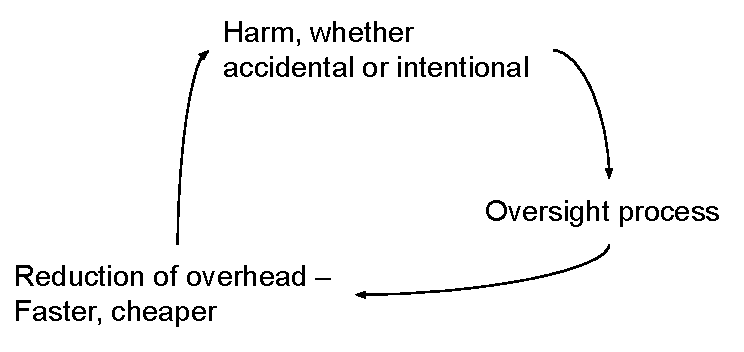
\includegraphics{images/process_loop_harm-oversight-improvement}
    \caption{loop: harm-oversight-improvement}
    \label{fig:harm-oversight-improvement}
\end{figure}








\subsection{TODO: Uncategorized}

Does a process exist?

% https://graphthinking.blogspot.com/2015/07/notes-on-bureaucracy-and-social-network.html
Do participants know about existing processes?

Processes can be undocumented. Then oral folklore is the mechanism. 


